\newpage
\section*{Conference Venue: Beurs van Berlage}

When you enter from the street (arrow in green, 1) and walk straight on, you will be in the Beursfoyer. To your right is the Grote Zaal ("zaal" stands for hall in Dutch; "kamer" stands for room). There, all breakfast, coffee breaks, lunches, afternoon demo/poster sessions as well as the PODS Reception on Sunday evening will be held. To your left are the Graanbeurszaal and the Effectenzaal. Both are large halls, of which the latter will be used for all plenary sessions. The other, smaller, rooms are upstairs.

~\\~

\begin{tabular}{p{.4\textwidth}p{.4\textwidth}}
\textbf{First floor}
\small
\begin{itemize}[noitemsep,topsep=0pt,parsep=0pt,partopsep=0pt]
\item[A.] Administratiezaal
\item[B.] Berlage zaal
\item[C.] Veilingzaal
\item[D.] Verwey kamer
\item[E.] Mendes da Costa kamer
\item[F.] Rode kamer
\item[G.] Blauwe kamer
\item[H.] Ontvangkamer
\item[I.] Roland Holst kamer
\item[J.] Derkinderen kamer
\item[K.] Zijl kamer
\end{itemize}
 & 
\textbf{Ground floor}
\small
\begin{itemize}[noitemsep,topsep=0pt,parsep=0pt,partopsep=0pt]
\item[L.] Grote Zaal
\item[M.] Effectenbeurszaal
\item[N.] Graanbeurszaal
\item[O.] Beursfoyer
\item[P.] Keurzaal
\end{itemize}
\end{tabular}

\newpage
~\\~~\\~~\\~

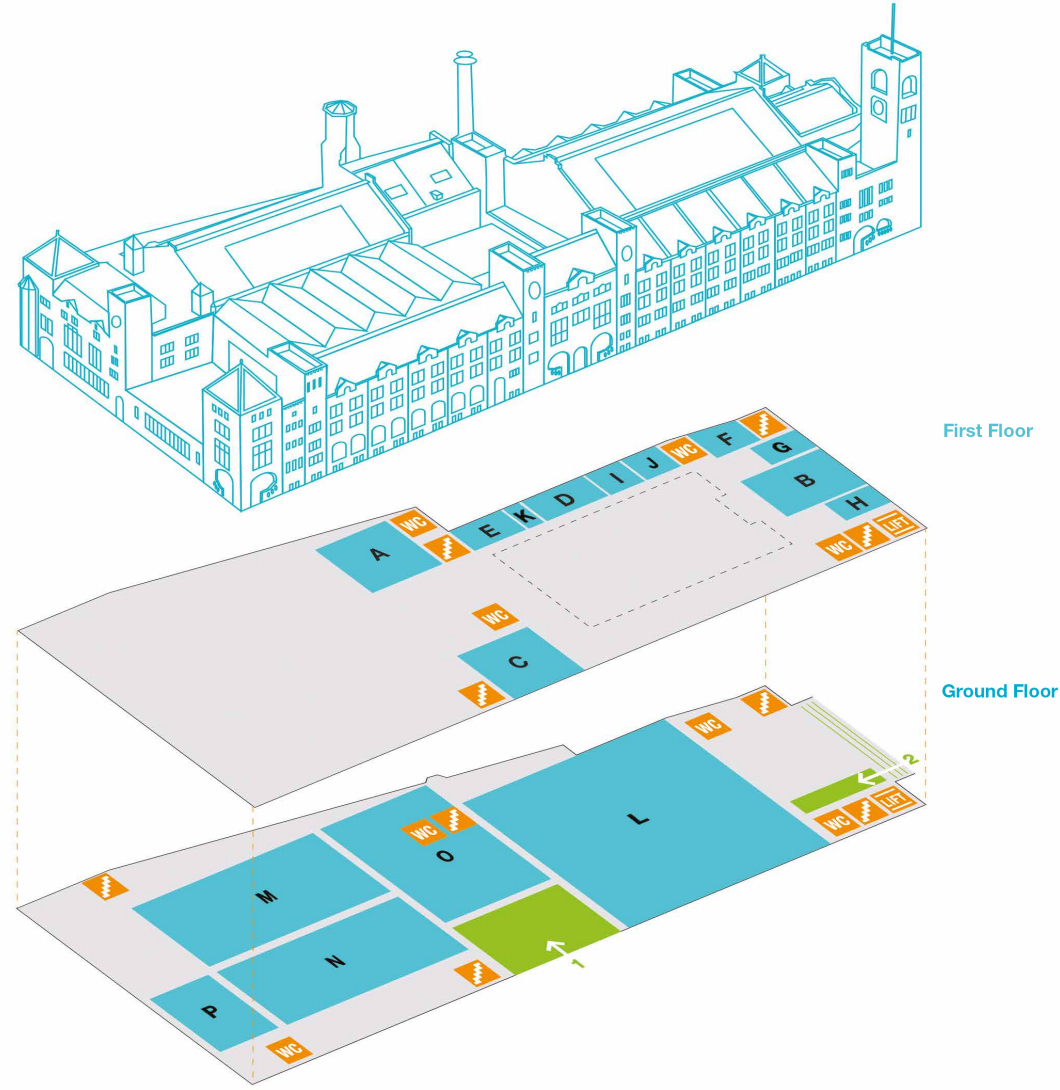
\includegraphics[width=\textwidth]{images/BerlageFloorplan.png}
